\documentclass[12pt,reqno,final,pdftex]{amsart}\usepackage[]{graphicx}\usepackage[]{color}
%% maxwidth is the original width if it is less than linewidth
%% otherwise use linewidth (to make sure the graphics do not exceed the margin)
\makeatletter
\def\maxwidth{ %
  \ifdim\Gin@nat@width>\linewidth
    \linewidth
  \else
    \Gin@nat@width
  \fi
}
\makeatother

\definecolor{fgcolor}{rgb}{0.345, 0.345, 0.345}
\newcommand{\hlnum}[1]{\textcolor[rgb]{0.686,0.059,0.569}{#1}}%
\newcommand{\hlstr}[1]{\textcolor[rgb]{0.192,0.494,0.8}{#1}}%
\newcommand{\hlcom}[1]{\textcolor[rgb]{0.678,0.584,0.686}{\textit{#1}}}%
\newcommand{\hlopt}[1]{\textcolor[rgb]{0,0,0}{#1}}%
\newcommand{\hlstd}[1]{\textcolor[rgb]{0.345,0.345,0.345}{#1}}%
\newcommand{\hlkwa}[1]{\textcolor[rgb]{0.161,0.373,0.58}{\textbf{#1}}}%
\newcommand{\hlkwb}[1]{\textcolor[rgb]{0.69,0.353,0.396}{#1}}%
\newcommand{\hlkwc}[1]{\textcolor[rgb]{0.333,0.667,0.333}{#1}}%
\newcommand{\hlkwd}[1]{\textcolor[rgb]{0.737,0.353,0.396}{\textbf{#1}}}%
\let\hlipl\hlkwb

\usepackage{framed}
\makeatletter
\newenvironment{kframe}{%
 \def\at@end@of@kframe{}%
 \ifinner\ifhmode%
  \def\at@end@of@kframe{\end{minipage}}%
  \begin{minipage}{\columnwidth}%
 \fi\fi%
 \def\FrameCommand##1{\hskip\@totalleftmargin \hskip-\fboxsep
 \colorbox{shadecolor}{##1}\hskip-\fboxsep
     % There is no \\@totalrightmargin, so:
     \hskip-\linewidth \hskip-\@totalleftmargin \hskip\columnwidth}%
 \MakeFramed {\advance\hsize-\width
   \@totalleftmargin\z@ \linewidth\hsize
   \@setminipage}}%
 {\par\unskip\endMakeFramed%
 \at@end@of@kframe}
\makeatother

\definecolor{shadecolor}{rgb}{.97, .97, .97}
\definecolor{messagecolor}{rgb}{0, 0, 0}
\definecolor{warningcolor}{rgb}{1, 0, 1}
\definecolor{errorcolor}{rgb}{1, 0, 0}
\newenvironment{knitrout}{}{} % an empty environment to be redefined in TeX

\usepackage{alltt}
%% DO NOT DELETE OR CHANGE THE FOLLOWING TWO LINES!
%% $Revision$
%% $Date$
\usepackage[round,sort,elide]{natbib}
\usepackage{graphicx}
\usepackage{times}
\usepackage{rotating}
\usepackage{subfig}
\usepackage{color}
\newcommand{\aak}[1]{\textcolor{cyan}{#1}}
\newcommand{\mab}[1]{\textcolor{red}{#1}}
\newcommand{\cec}[1]{\textcolor{blue}{#1}}

\setlength{\textwidth}{6.25in}
\setlength{\textheight}{8.75in}
\setlength{\evensidemargin}{0in}
\setlength{\oddsidemargin}{0in}
\setlength{\topmargin}{-.35in}
\setlength{\parskip}{.1in}
\setlength{\parindent}{0.3in}

%% cleveref must be last loaded package
\usepackage[sort&compress]{cleveref}
\newcommand{\crefrangeconjunction}{--}
\crefname{figure}{Fig.}{Figs.}
\Crefname{figure}{Fig.}{Figs.}
\crefname{table}{Table}{Tables}
\Crefname{table}{Tab.}{Tables}
\crefname{equation}{Eq.}{Eqs.}
\Crefname{equation}{Eq.}{Eqs.}
\crefname{appendix}{Appendix}{Appendices}
\Crefname{appendix}{Appendix}{Appendices}
\creflabelformat{equation}{#2#1#3}

\theoremstyle{plain}
\newtheorem{thm}{Theorem}
\newtheorem{corol}[thm]{Corollary}
\newtheorem{prop}[thm]{Proposition}
\newtheorem{lemma}[thm]{Lemma}
\newtheorem{defn}[thm]{Definition}
\newtheorem{hyp}[thm]{Hypothesis}
\newtheorem{example}[thm]{Example}
\newtheorem{conj}[thm]{Conjecture}
\newtheorem{algorithm}[thm]{Algorithm}
\newtheorem{remark}{Remark}
\renewcommand\thethm{\arabic{thm}}
\renewcommand{\theremark}{}

\numberwithin{equation}{part}
\renewcommand\theequation{\arabic{equation}}
\renewcommand\thesection{\arabic{section}}
\renewcommand\thesubsection{\thesection.\arabic{subsection}}
\renewcommand\thefigure{\arabic{figure}}
\renewcommand\thetable{\arabic{table}}
\renewcommand\thefootnote{\arabic{footnote}}

\newcommand\scinot[2]{$#1 \times 10^{#2}$}
\newcommand{\code}[1]{\texttt{#1}}
\newcommand{\pkg}[1]{\textsf{#1}}
\newcommand{\dlta}[1]{{\Delta}{#1}}
\newcommand{\Prob}[1]{\mathbb{P}\left[#1\right]}
\newcommand{\Expect}[1]{\mathbb{E}\left[#1\right]}
\newcommand{\Var}[1]{\mathrm{Var}\left[#1\right]}
\newcommand{\dd}[1]{\mathrm{d}{#1}}
\newcommand{\citetpos}[1]{\citeauthor{#1}'s \citeyearpar{#1}}
\IfFileExists{upquote.sty}{\usepackage{upquote}}{}
\begin{document}



In this document, I explore the methods used by GEMs for generating offspring.

Here is the code for generating new individuals.
\begin{knitrout}\scriptsize
\definecolor{shadecolor}{rgb}{0.969, 0.969, 0.969}\color{fgcolor}\begin{kframe}
\begin{alltt}
\hlcom{## Code for generating new individuals}
\hlstd{pick_individuals} \hlkwb{<-} \hlkwa{function}\hlstd{(}\hlkwc{N0}\hlstd{,} \hlkwc{traitmean}\hlstd{,} \hlkwc{traitsd}\hlstd{) \{}
    \hlstd{mu} \hlkwb{<-} \hlkwd{log}\hlstd{(traitmean}\hlopt{^}\hlnum{2} \hlopt{/} \hlkwd{sqrt}\hlstd{((traitsd)}\hlopt{^}\hlnum{2}\hlopt{+}\hlstd{traitmean}\hlopt{^}\hlnum{2}\hlstd{))}
    \hlstd{sigma} \hlkwb{<-} \hlkwd{sqrt}\hlstd{(}\hlkwd{log}\hlstd{(traitsd}\hlopt{^}\hlnum{2}\hlopt{/}\hlstd{traitmean}\hlopt{^}\hlnum{2} \hlopt{+} \hlnum{1}\hlstd{))}
    \hlcom{## record this initial distribution in the output}
    \hlkwd{return}\hlstd{(}\hlkwd{rlnorm}\hlstd{(N0,} \hlkwc{meanlog}\hlstd{=mu,} \hlkwc{sdlog}\hlstd{=sigma))}
\hlstd{\}}
\end{alltt}
\end{kframe}
\end{knitrout}

I am going to generate an initial population of ``parents'' with identical traits.
To do this, I am using the pick\_individuals function with N0=1000, traitmean=1, and traitsd=0.3.
Each of these parents will give birth to a single offspring.
Offspring generation in GEMs is a bit complex.
In particular, given a parent with trait $p$ and a population of parents with mean trait $\bar{p}$, and a heritability of $h^2$, the value of traitmean that will be plugged into pick\_individuals is $(1-h^2)\bar{p} + h^2p$.
At the extremes, if $h^2=1$ then the mean trait in the offspring generation function is identical to their parent trait; if $h^2=0$, then the mean trait in the offspring generation function is equal to the population-level mean.
The value of traitsd is calculated using $\sqrt{1-(h^2)^2}\left((1-h^2)*\sigma_0 + h^2\sigma_p\right)$, where $\sigma_0$ was the initial amount of trait variation and $\sigma_p$ is the trait variation in the current population.
Starting out, then, $\sigma_0 = \sigma_p$.

What I am going to do is generating one offspring per parent for 10 different levels of heritability ranging from 0.1 to 1.0.
That gives me data upon which I calculate a parent-offspring regression, which is a standard way of estimating heritability in real data: heritability is the slope of the parent-offspring regression.
I repeat this process, using the offspring from the first generation as parents for a second generation, and then again performing a parent-offspring regression.
Finally, just for completeness, I do this for a third generation, using the offspring of the second generation as parents.
The three figures show the estimates of heritability across the generations.


\begin{knitrout}\scriptsize
\definecolor{shadecolor}{rgb}{0.969, 0.969, 0.969}\color{fgcolor}\begin{figure}

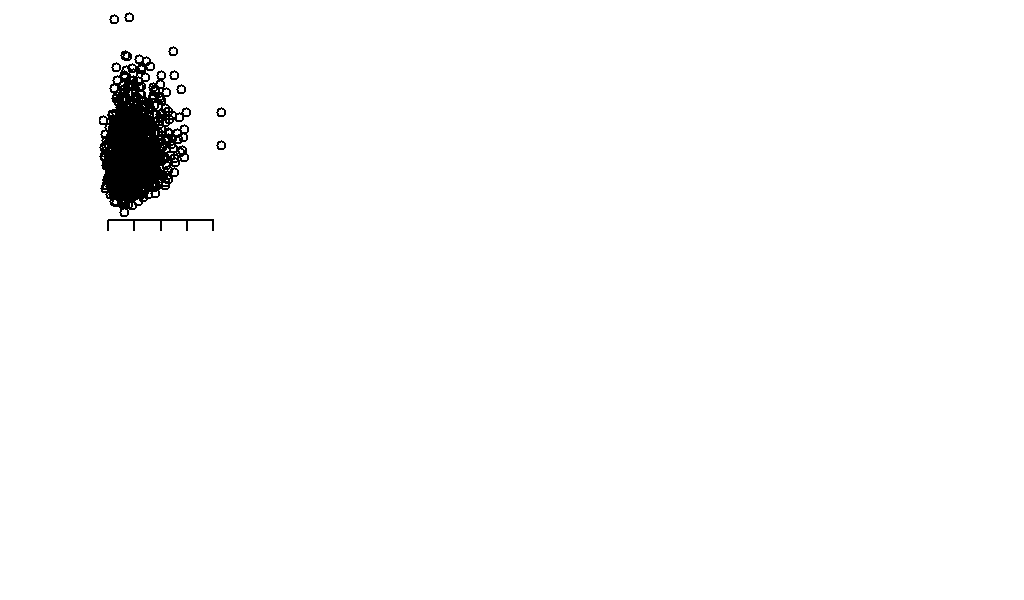
\includegraphics[width=\linewidth]{figure/unnamed-chunk-2-1} \hfill{}

\caption[Parent-offspring regressions for the first generation]{Parent-offspring regressions for the first generation.}\label{fig:unnamed-chunk-2}
\end{figure}


\end{knitrout}

\begin{knitrout}\scriptsize
\definecolor{shadecolor}{rgb}{0.969, 0.969, 0.969}\color{fgcolor}\begin{figure}

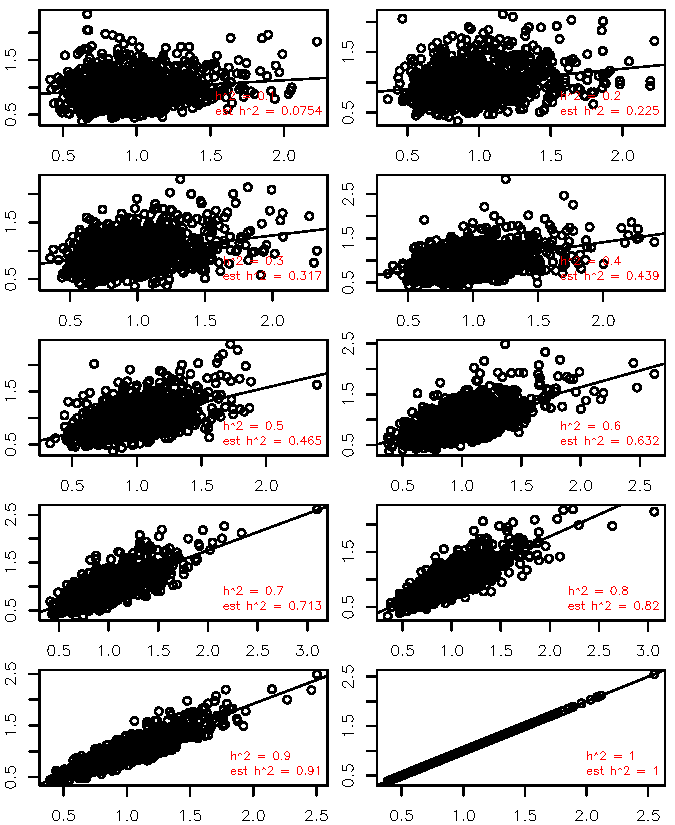
\includegraphics[width=\linewidth]{figure/unnamed-chunk-3-1} \hfill{}

\caption[Parent-offspring regressions for the second generation]{Parent-offspring regressions for the second generation.}\label{fig:unnamed-chunk-3}
\end{figure}


\end{knitrout}

\begin{knitrout}\scriptsize
\definecolor{shadecolor}{rgb}{0.969, 0.969, 0.969}\color{fgcolor}\begin{figure}

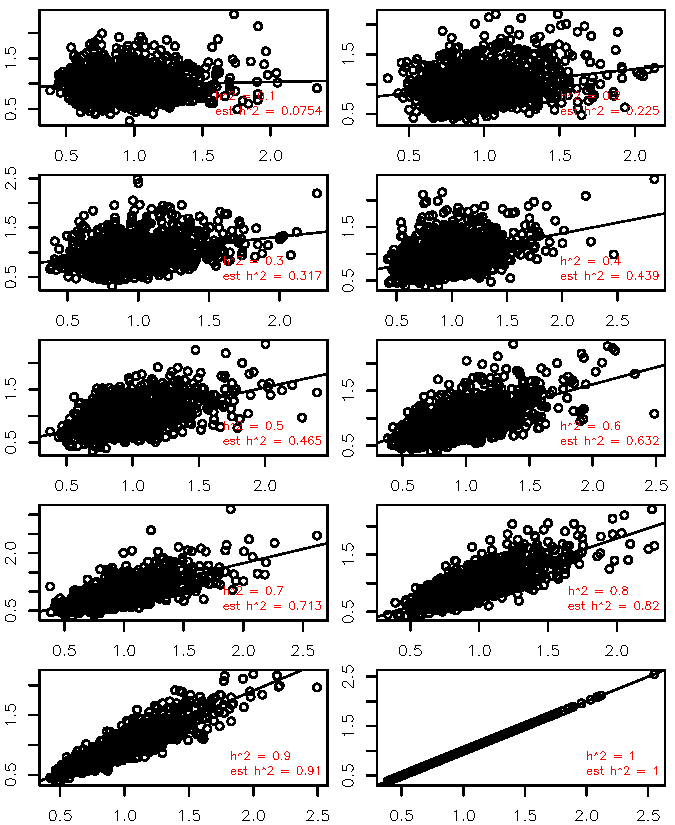
\includegraphics[width=\linewidth]{figure/unnamed-chunk-4-1} \hfill{}

\caption[Parent-offspring regressions for the third generation]{Parent-offspring regressions for the third generation.}\label{fig:unnamed-chunk-4}
\end{figure}


\end{knitrout}

\newpage

Let's compare that to the case where I'm actually running a GEM to see what happens.
In particular, I want to study how the parent-offspring regression changes at different timepoints, and to compare these to the regression over the entire simulation run, which is something I have looked at in the past (the fact that this ``overall'' parent-offspring regression has a slope that is very close to 1 is what has sent me down this rabbit hole in the first place).
You can see that, if you examine the regression over the entire simulation run, the heritability appears to be very high, examined over any smaller interval, it is exactly where you expect it to be!
This is because, if you look over the entire simulation run, you are looking at literally tens of thousands of data points, spread over a wide phenotypic range.
That is the key: the fact that the parent-offspring regression intercept is moving as the population evolves.
At the whole-simulation scale, what you are really seeing is a bunch of parent-offspring regressions from different time points stacked up next to each other.
At that scale, the relationship between parents and offspring will start to look one-to-one, even though the actual parent-offspring regression for any particular set of parents alive at one time has a slope that is well predicted by the supplied heritability value.

\begin{knitrout}\scriptsize
\definecolor{shadecolor}{rgb}{0.969, 0.969, 0.969}\color{fgcolor}\begin{figure}

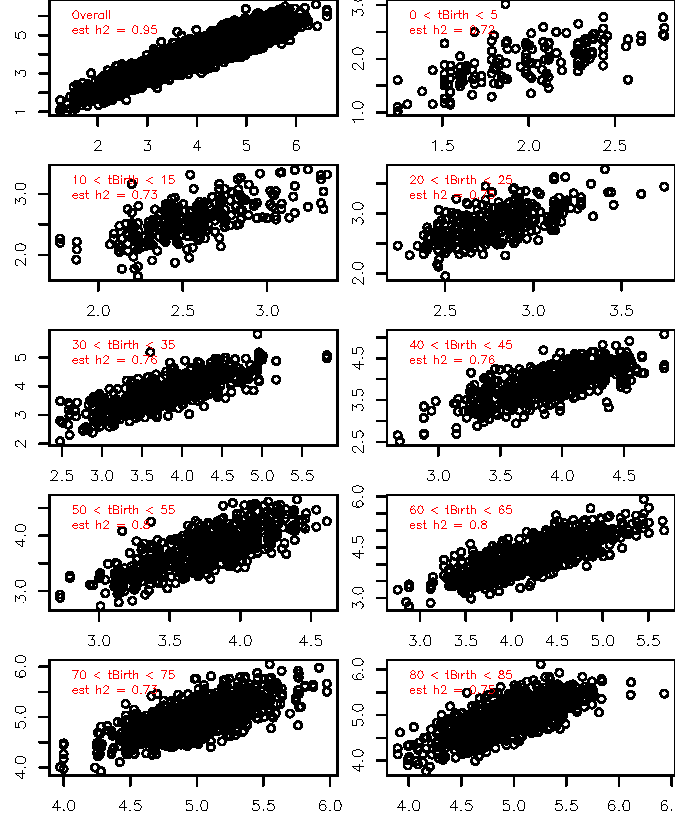
\includegraphics[width=\linewidth]{figure/unnamed-chunk-5-1} \hfill{}

\caption[Parent-offspring regressions from a GEM simulation with h2=0.9]{Parent-offspring regressions from a GEM simulation with h2=0.9.}\label{fig:unnamed-chunk-5}
\end{figure}


\end{knitrout}


\begin{knitrout}\scriptsize
\definecolor{shadecolor}{rgb}{0.969, 0.969, 0.969}\color{fgcolor}\begin{figure}

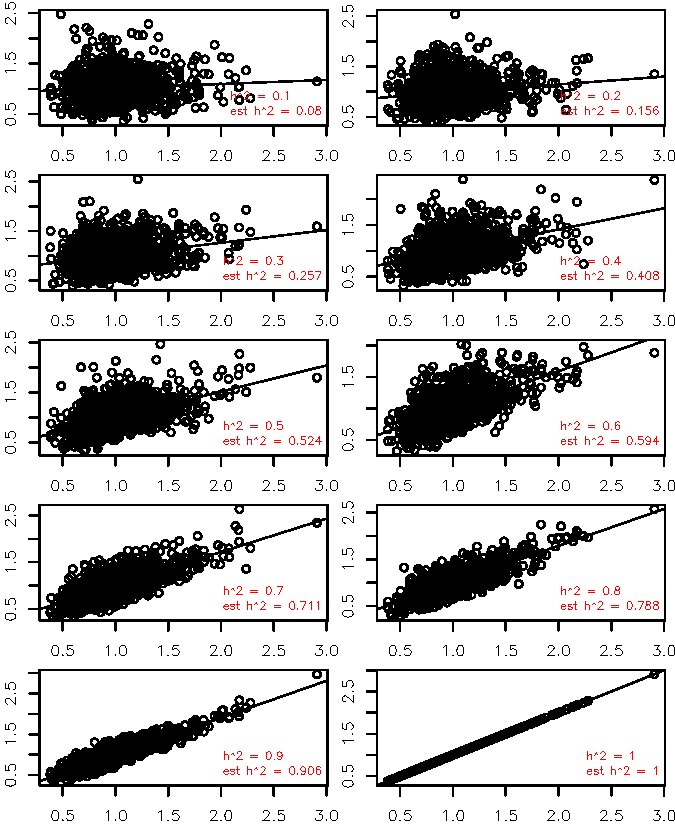
\includegraphics[width=\linewidth]{figure/unnamed-chunk-6-1} \hfill{}

\caption[Parent-offspring regressions from a GEM simulation with h2=0.7]{Parent-offspring regressions from a GEM simulation with h2=0.7.}\label{fig:unnamed-chunk-6}
\end{figure}


\end{knitrout}



\begin{knitrout}\scriptsize
\definecolor{shadecolor}{rgb}{0.969, 0.969, 0.969}\color{fgcolor}\begin{figure}

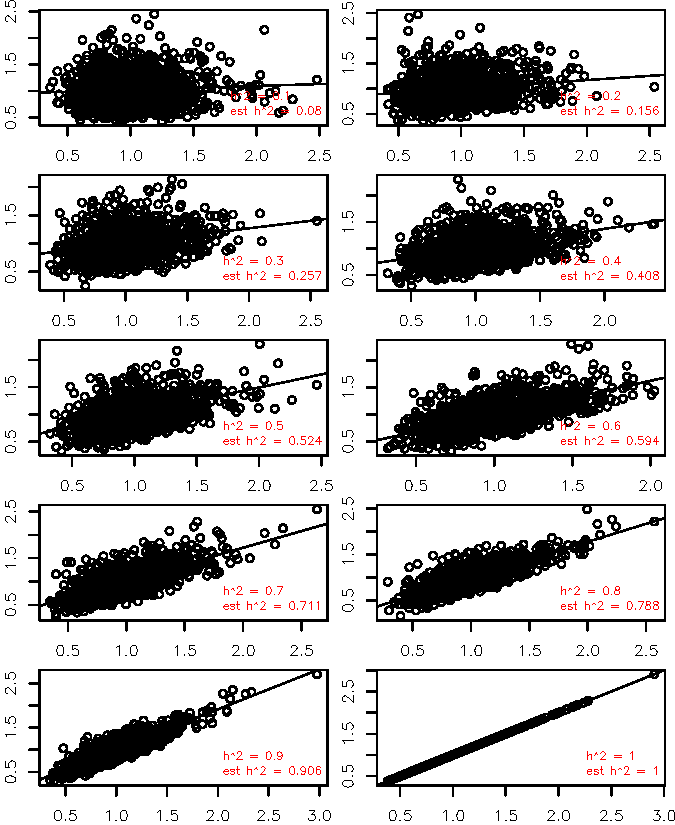
\includegraphics[width=\linewidth]{figure/unnamed-chunk-7-1} \hfill{}

\caption[Parent-offspring regressions from a GEM simulation with h2=0.5]{Parent-offspring regressions from a GEM simulation with h2=0.5.}\label{fig:unnamed-chunk-7}
\end{figure}


\end{knitrout}

\begin{knitrout}\scriptsize
\definecolor{shadecolor}{rgb}{0.969, 0.969, 0.969}\color{fgcolor}\begin{figure}

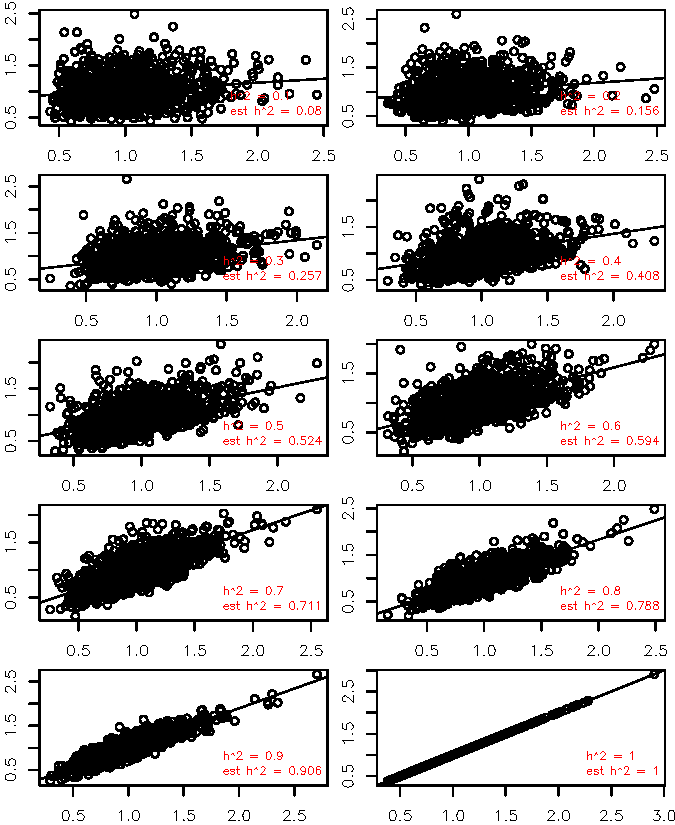
\includegraphics[width=\linewidth]{figure/unnamed-chunk-8-1} \hfill{}

\caption[Parent-offspring regressions from a GEM simulation with h2=0.3]{Parent-offspring regressions from a GEM simulation with h2=0.3.}\label{fig:unnamed-chunk-8}
\end{figure}


\end{knitrout}



\end{document}


